\documentclass{beamer}
\usetheme{Pittsburgh}
\beamertemplatenavigationsymbolsempty


\usepackage{amsmath}
\usepackage{amssymb}
\usepackage{bm} % For bold math symbols
\usepackage{graphicx}
\usepackage{tikz}



\usepackage{subfig} % Changed from subfigure (deprecated)
\usepackage{multirow}
\usepackage{multicol}
\usepackage{color}
\usepackage{url}
\usepackage{hyperref}
\usepackage{listings}
\usepackage[noend]{algorithm}
\usepackage{physics} 

\usepackage{animate}

% add image path
\graphicspath{{Images/}}






\DeclareMathOperator{\argmin}{argmin}
\DeclareMathOperator{\argmax}{argmax}






\title{Weekly Updates\\
\tiny{Friday, 25/04/2025}}
\author{Andrea Bonifacio}
\date{}

\begin{document}

\begin{frame}
\titlepage
\end{frame}


\begin{frame}{Where are we?}
    \begin{itemize}
        \item I have a fully working pipeline from linear modes extraction in SOFA to the training of the neural network to validate the results in SOFA.
        \item I have removed the origin constraint from the energy calculation, zeroing the bias in the neural network, and observed no significant difference in the results.
        \item I added a boundary constraint to the loss function, since the network wasn't respecting the boundary conditions.
        \item It seems that the prediction of the network is not orthogonal between the modes, and doesn't reflect what stated in the paper.
    \end{itemize}
\end{frame}

\begin{frame}
    \frametitle{Correlation of Linear Modes}
    
    \begin{itemize}
        \item \textbf{Goal:} Verify the orthogonality of the pre-computed linear modes $\mathbf{\Phi}$.
        \item \textbf{Linear Displacement:} The displacement based only on linear modes is $\mathbf{l}(\mathbf{z}) = \mathbf{\Phi} \mathbf{z}$.
        \item \textbf{Direction Vectors:} We consider the direction of change in linear displacement when perturbing a single latent coordinate $z_i$ from the origin ($\mathbf{z}=\mathbf{0}$):
        \[
            \mathbf{e}_i^{\text{linear}} = \frac{\partial \mathbf{l}}{\partial z_i} \bigg|_{\mathbf{z}=\mathbf{0}} = \mathbf{\Phi}_i 
        \]
        (where $\mathbf{\Phi}_i$ is the $i$-th column/mode vector of $\mathbf{\Phi}$)
        \item \textbf{Correlation Matrix:} We compute the matrix of dot products between these direction vectors:
        \[
            \mathbf{C}^{\text{linear}}[i, j] = (\mathbf{e}_i^{\text{linear}})^T \mathbf{e}_j^{\text{linear}} = \mathbf{\Phi}_i^T \mathbf{\Phi}_j
        \]
    \end{itemize}
    
\end{frame}

\begin{frame}
    \frametitle{Correlation of Linear Modes}
    
    \begin{figure}
        \centering
        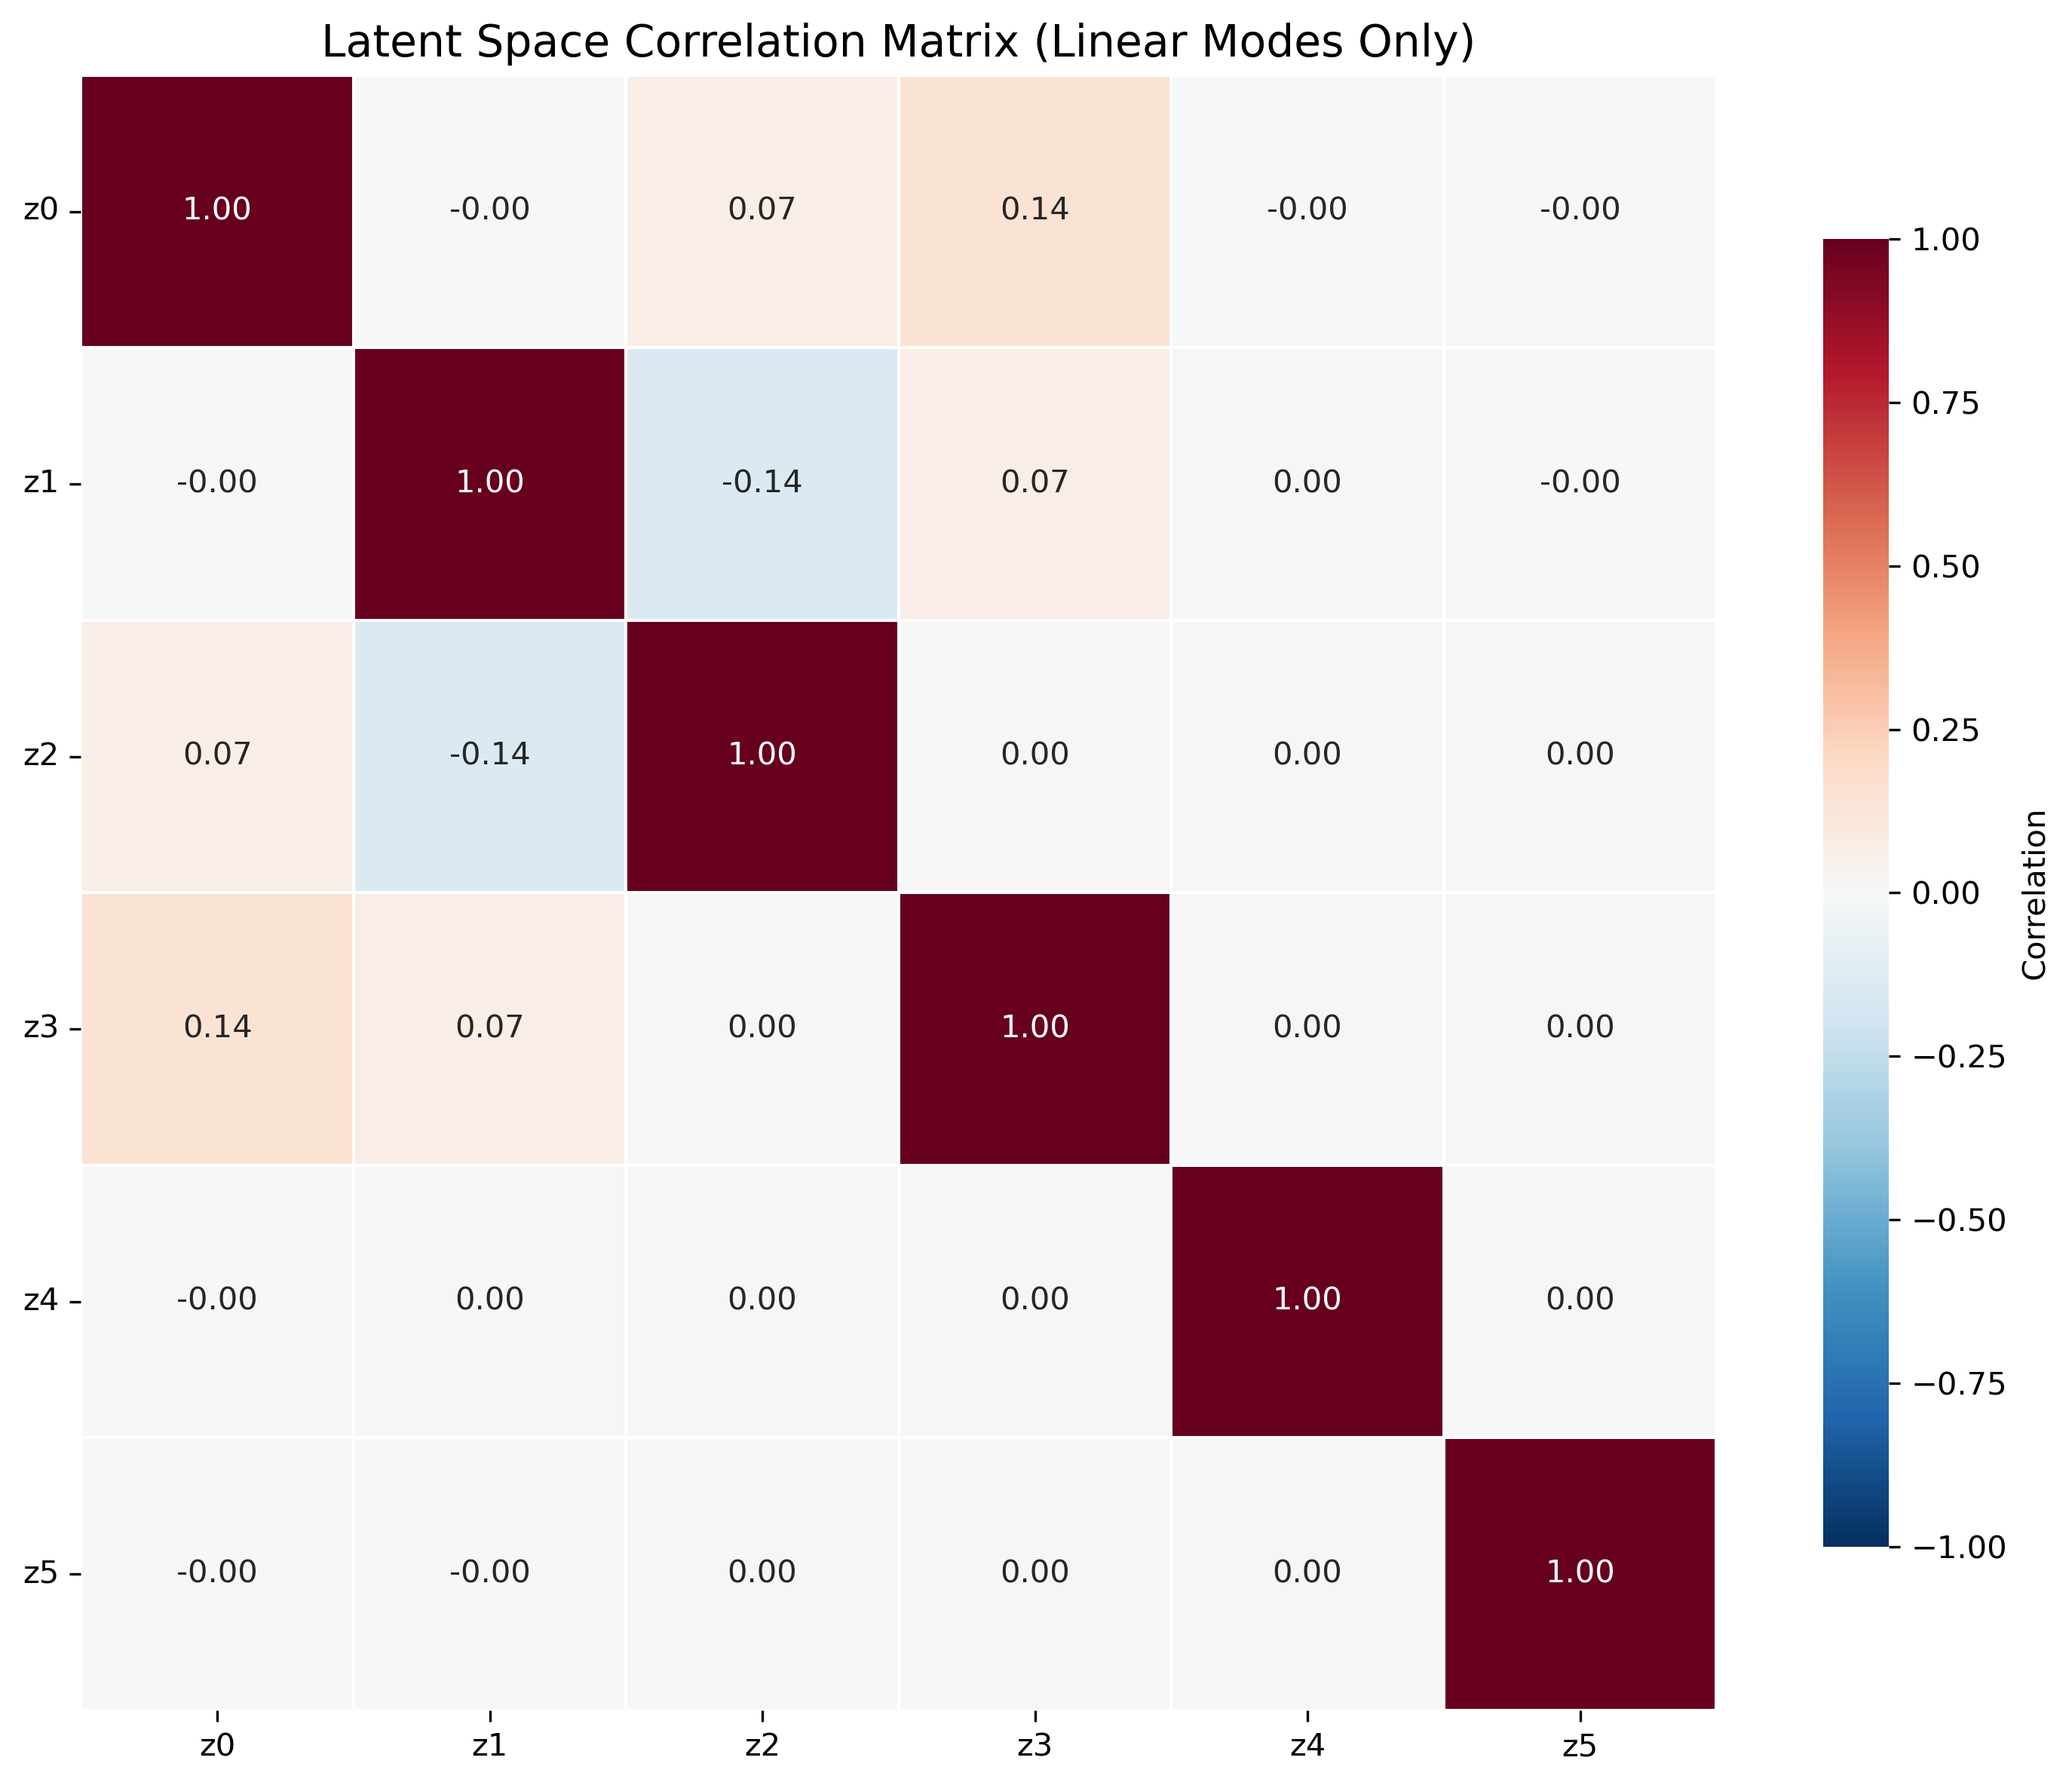
\includegraphics[width=0.7\textwidth]{Images/latent_correlations_linear_linear.png}
        \caption{Correlation of linear modes.}
        \label{fig:linear_correlation}

    \end{figure}
    \end{frame}

\begin{frame}
    \frametitle{Correlation of Latent Space}
    
    \begin{itemize}
        \item \textbf{Total Displacement:} $\mathbf{u}(\mathbf{z}) = \mathbf{l}(\mathbf{z}) + \mathbf{y}(\mathbf{z}) = \mathbf{\Phi} \mathbf{z} + \text{NN}(\mathbf{z})$
        \item \textbf{Direction Vectors:} We define effective direction vectors at the origin as the gradient of the \textit{total} displacement w.r.t. each latent coordinate:
        \[
            \mathbf{e}_i^{\text{total}} = \frac{\partial \mathbf{u}}{\partial z_i} \bigg|_{\mathbf{z}=\mathbf{0}}
        \]
        \item \textbf{Finite Difference Approximation:} We approximate this gradient:
        \[
            \mathbf{e}_i^{\text{total}} \approx \frac{\mathbf{u}(\boldsymbol{\delta}_i) - \mathbf{u}(\mathbf{0})}{\delta}
        \]
        where $\boldsymbol{\delta}_i$ is a vector with a small value $\delta$ at index $i$ and zeros elsewhere.
        (Note: If $\text{NN}(\mathbf{0})=\mathbf{0}$, then $\mathbf{u}(\mathbf{0})=\mathbf{0}$)
        \item \textbf{Correlation Matrix:} Compute dot products:
        \[
            \mathbf{C}^{\text{total}}[i, j] = (\mathbf{e}_i^{\text{total}})^T \mathbf{e}_j^{\text{total}}
        \]

    \end{itemize}
    
    \end{frame}

\begin{frame}
    \frametitle{Correlation of Latent Space}
    
    \begin{figure}
        \centering
        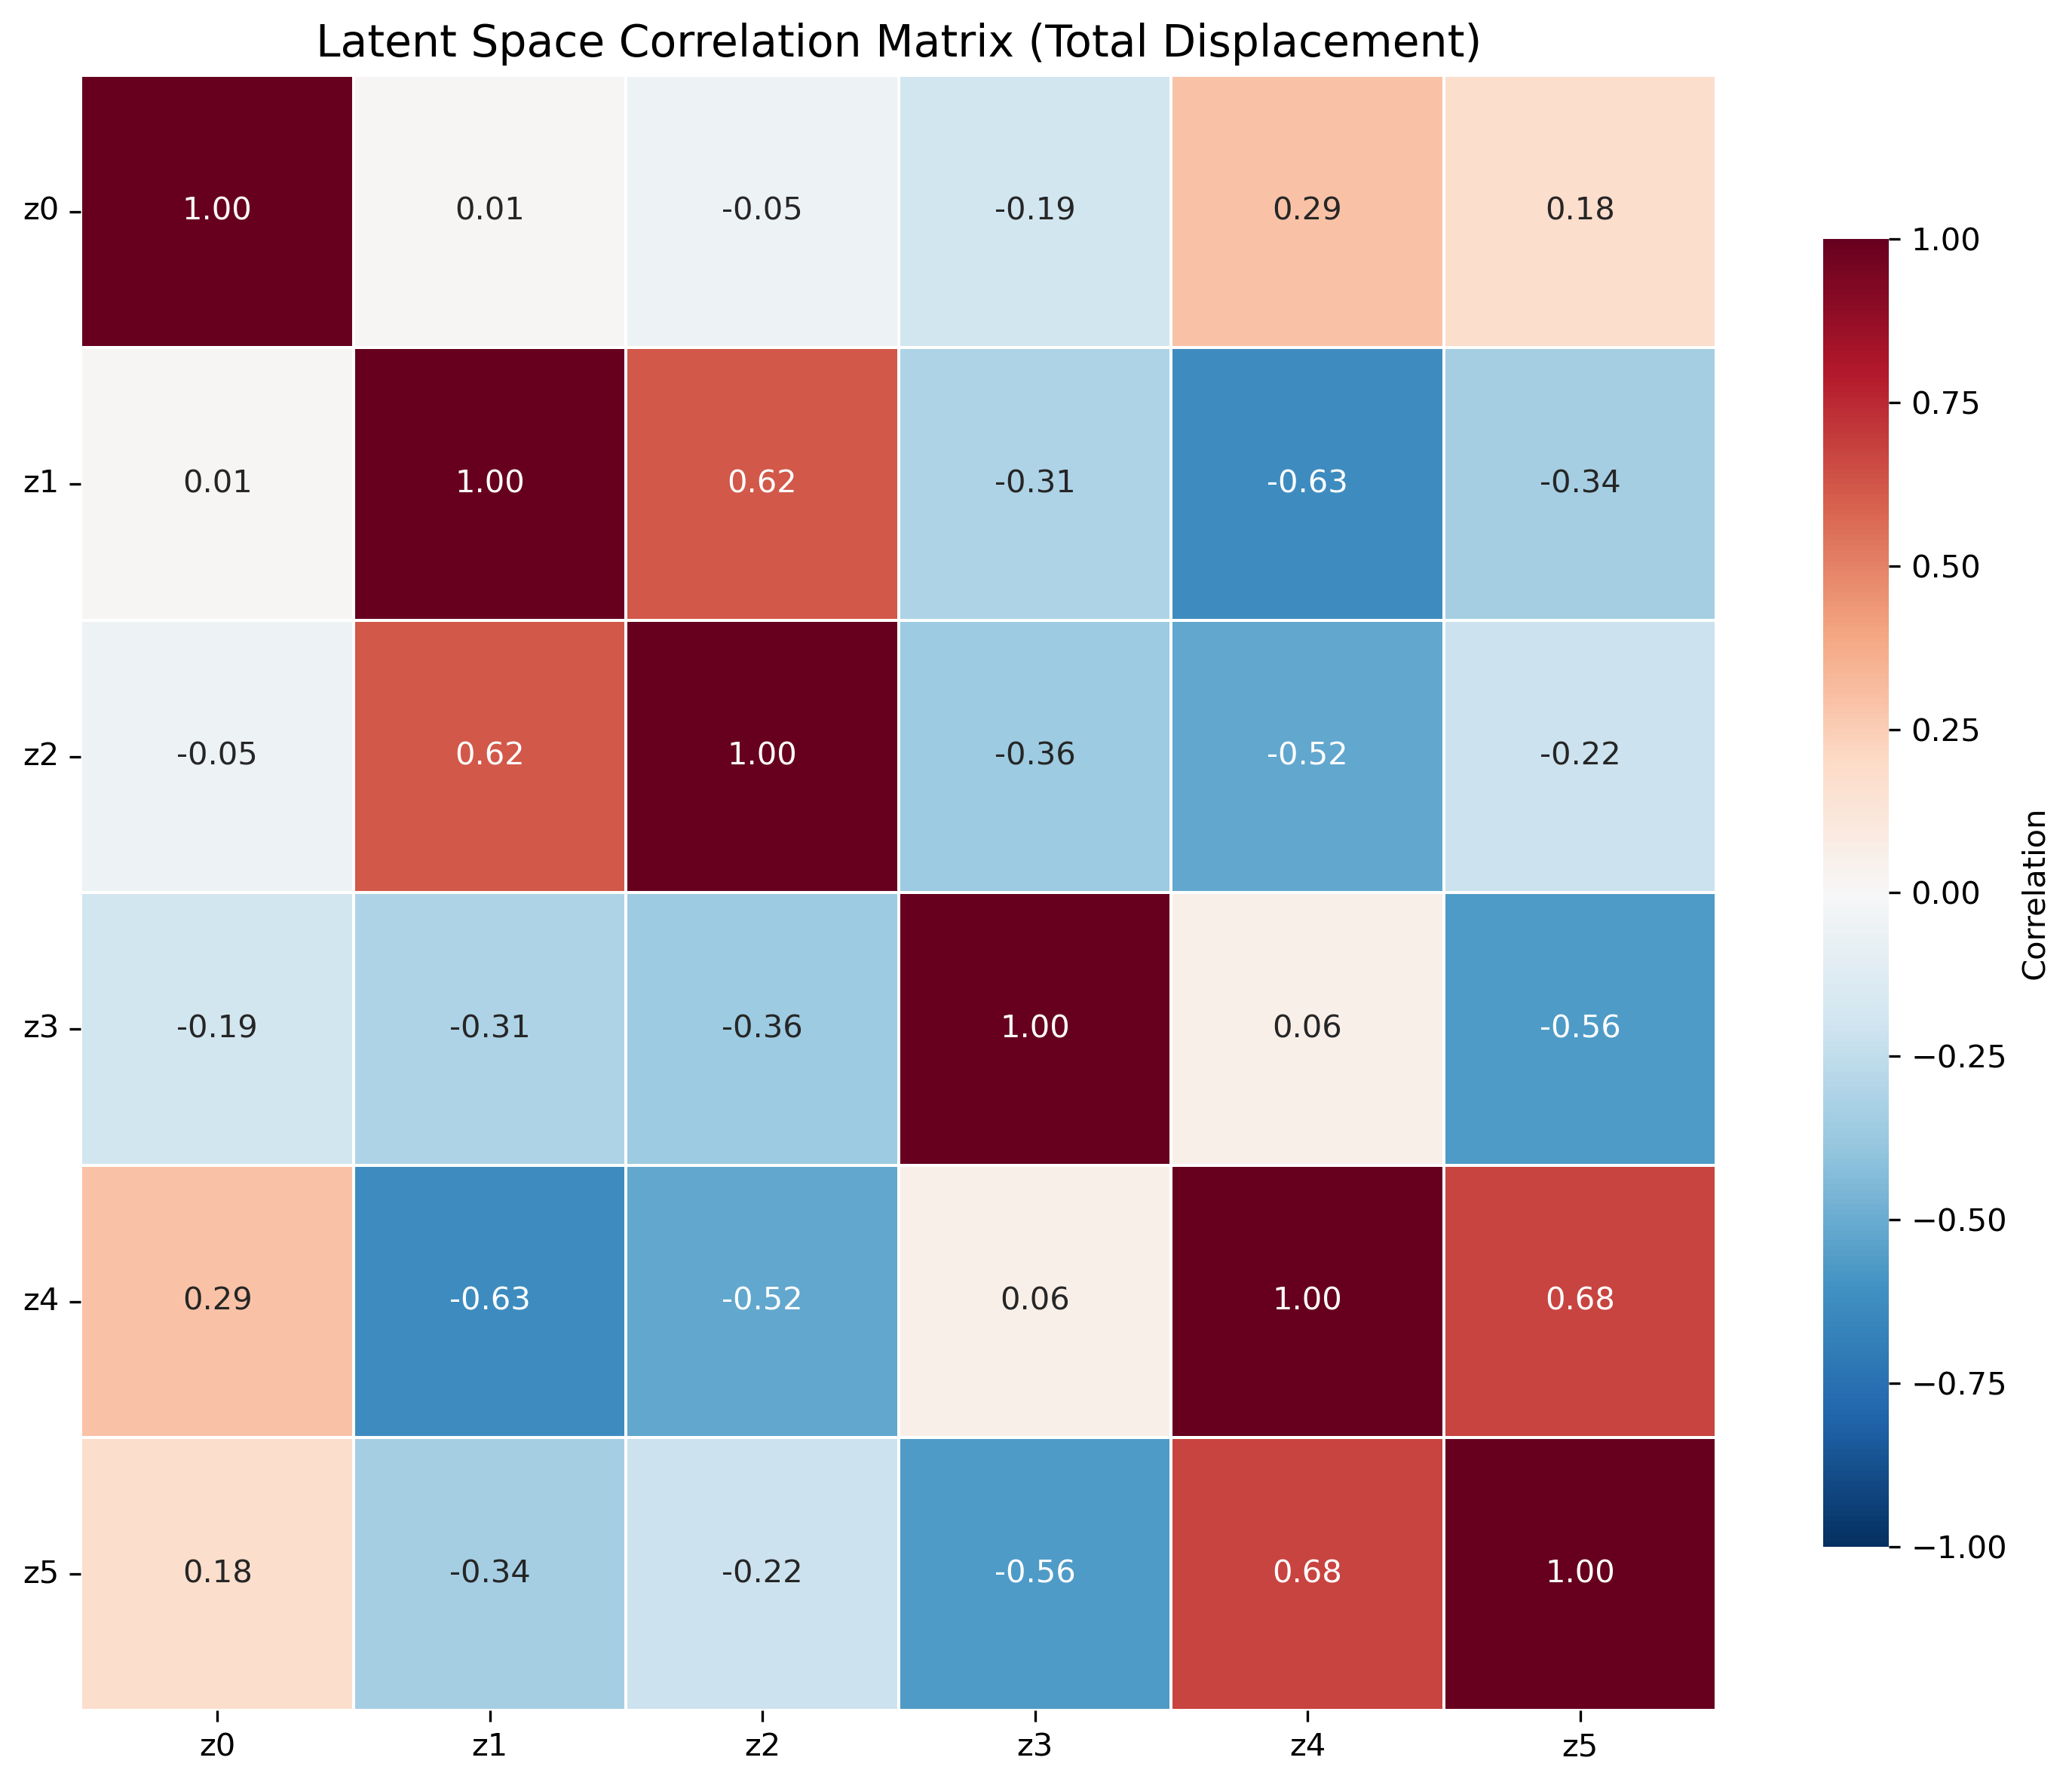
\includegraphics[width=0.7\textwidth]{Images/latent_correlations_total_total.png}
        \caption{Correlation of latent space.}
        \label{fig:latent_correlation}

    \end{figure}
\end{frame}




\begin{frame}
    \frametitle{Validation Static Case}
    \begin{itemize}
        \item In the paper they state that there is not a limit on training epochs, they use more than 20k epochs for the armadillo.
        \item I noticed the same behavior while training on the beam mesh. I stopped it at 500 epochs, but the loss was still decreasing. 
        \item As a metric to check the training, I use the reduction in energy w.r.t. the energy of the linear modes.
        \item In the last training, I stopped it at around 98\% of the energy reduction.
    \end{itemize}
\end{frame}

\begin{frame}
    \frametitle{Validation Static Case}
    
    \begin{figure}
        \centering
        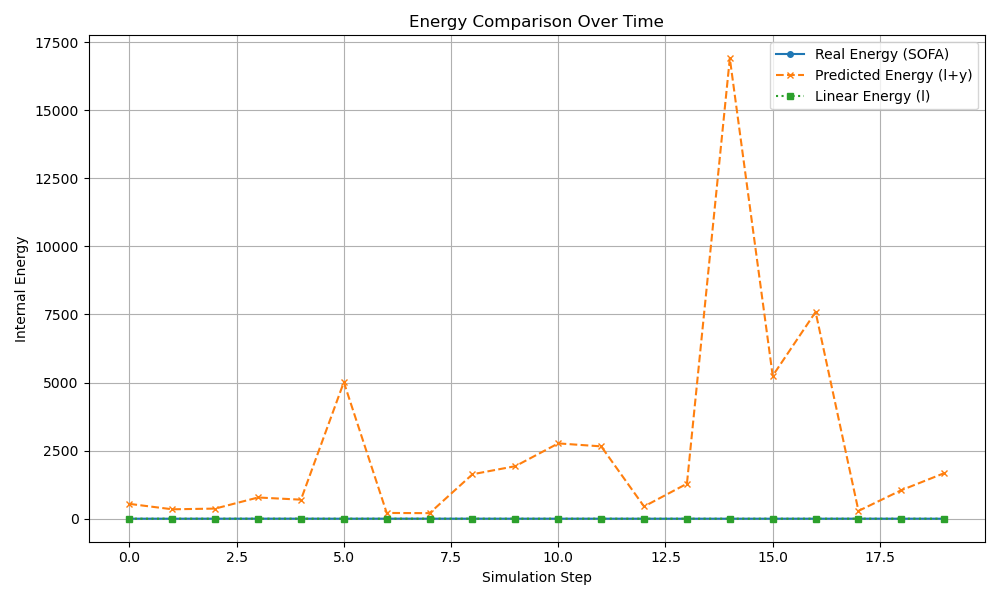
\includegraphics[width=0.8\textwidth]{Images/energy_comparison.png}
        \caption{Energy comparison between linear modes and neural network.}
        \label{fig:energy_comparison}
    \end{figure}

    \end{frame}
\begin{frame}
    \frametitle{Validation Static Case}
    
    \begin{itemize}
        \item The energy is computed for all the three cases: linear modes, neural network, and the reference solution using the energy calculator of the neural network.
        \item While during the training, the energy of the neural modes is much lower than the one of the linear modes, when validating the results, linear modes have a much lower energy.
        \item This could mean that the network is not generalizing well, or that my simulations are exhibiting very little nonlinear behavior. (It could be, since I am just applying a small force to the end of the beam)
    \end{itemize}
\end{frame}
% Q&A
\begin{frame}
    \begin{center}
        \color{blue} \Huge{Questions?}
    \end{center}

\end{frame}
\end{document}

